% ===
%
% Official LaTeX seminar report template of the
% Chair for AI Methodology (AIM)
% RWTH Aachen University, Aachen, Germany
%
% Author: Jakob Bossek (bossek@aim.rwth-aachen.de)
%
% AIM website: https://aim.rwth-aachen.de/
%
% ===

% The 'review' option activates line numbering
\documentclass[review]{AIM_report}

% includes/preamble.tex is the right place to add new packages etc.
% tables
\RequirePackage{booktabs}
\RequirePackage{colortbl}
\RequirePackage{multicol}
\RequirePackage{multirow}
\RequirePackage{xspace}
\RequirePackage[final]{pdfpages}

% \smiley{} and \frowney{}
\RequirePackage{wasysym}

% quotation
\RequirePackage{csquotes}


% import commenting macros
\input{includes/macros/commenting}
\definecolor{classColor}{RGB}{0,0,139}    % Dark Blue for classes
\definecolor{methodColor}{RGB}{63,92,161} % Darker Turquoise for methods
\definecolor{typeColor}{RGB}{139,0,0}  % Dark Red for types
\definecolor{commentColor}{RGB}{34,139,34} % ForestGreen for comments
\definecolor{variableColor}{RGB}{0,139,139} % Slightly darker Turquoise for variables
\definecolor{libraryColor}{RGB}{0,0,0} % Black for libraries

% Define Rust as a custom language
\lstdefinelanguage{Rust}{
    keywords={abstract, alignof, as, become, box, break, const, continue, crate, do, else, enum, extern, false, final, fn, for, if, impl, in, let, loop, macro, match, mod, move, mut, offsetof, override, priv, proc, pub, pure, ref, return, Self, self, sizeof, static, struct, super, trait, true, type, typeof, unsafe, unsized, use, virtual, where, while, yield},
    morecomment=[l]{//},
    morecomment=[s]{/*}{*/},
    morestring=[b]",
    morestring=[b]',
}

\lstdefinestyle{python}{
    language=Python,
    basicstyle=\ttfamily\small,
    keywordstyle=\color{blue},
    commentstyle=\color{commentColor},
    stringstyle=\color{red},
    morekeywords={self, None, True, False, import, from, as, def, class, return, if, elif, else, for, while, break, continue, pass, try, except, finally, raise},
    showstringspaces=false,
    % Custom highlighting for classes, variables and methods
    classoffset=4, % Offset for variable styling
    morekeywords={forecasting_data_set, forecasting_data_set_res, classification_data_set, classification_data_set_res, dataset, dataset_type, past_window, future_horizon, stride, labels, batch_size, num_workers, downsampling_rate, impute_strategy, splitting_strategy, splitting_ratios}, % List of variables
    keywordstyle=\color{variableColor},
    classoffset=3, % Separate class styling
    morekeywords={ForecastingDataSet, ClassificationDataSet, DatasetType, ImputeStrategy, SplittingStrategy}, % List of classes
    keywordstyle=\color{classColor},
    classoffset=2, % Reset for methods
    morekeywords={impute, downsample, split, normalize, standardize, collect, __init__}, % List of methods
    keywordstyle=\color{methodColor},
    classoffset=1, % Reset for types
    morekeywords={np, ndarray, LeaveNaN, Temporal},
    keywordstyle=\color{typeColor},
    showstringspaces=false,
}

\lstdefinestyle{rust}{
    language=Rust,
    basicstyle=\ttfamily\small,
    keywordstyle=\color{blue},
    commentstyle=\color{commentColor},
    stringstyle=\color{red},
    showstringspaces=false,
    % Custom highlighting for classes, variables and methods
    classoffset=3, % Offset for variable styling
    morekeywords={train_view, val_view, test_view, self, _py, train_data, val_data, test_data, data, train_split_index, val_split_index}, % List of variables
    keywordstyle=\color{variableColor},
    classoffset=2, % Separate class styling
    morekeywords={ArrayBase, Dim, PyResult, DataMut, Elem, S, Ok, Python, SplittingStrategy}, % List of classes
    keywordstyle=\color{classColor},
    classoffset=1, % Reset for methods
    morekeywords={impute, downsample, split, normalize, standardize, collect, as_mut, unwrap, get_split_views_mut, check_arrays_set}, % List of methods
    keywordstyle=\color{methodColor},
    showstringspaces=false,
}

% generics
\newcommand{\rustCode}[3]{\texttt{\textcolor{#2}{#1}#3}\xspace}
\newcommand{\rustFunc}[2]{\rustCode{#1}{methodColor}{(\textcolor{variableColor}{#2})}}
\newcommand{\rustNoArgsFunc}[1]{\rustFunc{#1}{}}
\newcommand{\rustClass}[2]{\rustCode{#1}{classColor}{#2}}
\newcommand{\rustGenClass}[1]{\rustClass{#1}{<...>}}
\newcommand{\rustNoArgsClass}[1]{\rustClass{#1}{}}
\newcommand{\rustVar}[1]{\rustCode{#1}{variableColor}{}}
\newcommand{\rustLibrary}[1]{\rustCode{#1}{libraryColor}{}}

% functions
\newcommand{\impute}{\rustNoArgsFunc{impute}}
\newcommand{\downsample}{\rustNoArgsFunc{downsample}}
\newcommand{\downsampleFac}{\rustFunc{downsample}{factor}}
\newcommand{\splitShort}{\rustNoArgsFunc{split}}
\newcommand{\splitFore}{\rustFunc{split}{train\_part, val\_part, test\_part}}
\newcommand{\normalize}{\rustNoArgsFunc{normalize}}
\newcommand{\standardize}{\rustNoArgsFunc{standardize}}
\newcommand{\collect}{\rustNoArgsFunc{collect}}
\newcommand{\collectFore}{\rustFunc{collect}{past\_window, future\_horizon, stride}}
\newcommand{\setup}{\rustNoArgsFunc{setup}}

% classes
\newcommand{\arraybase}{\rustGenClass{ArrayBase}}
\newcommand{\arrayrust}{\rustGenClass{Array}}
\newcommand{\arrayview}{\rustGenClass{ArrayView}}
\newcommand{\py}{\rustGenClass{Py}}
\newcommand{\classificationDataSet}{\rustNoArgsClass{ClassificationDataSet}}
\newcommand{\forecastingDataSet}{\rustNoArgsClass{ForecastingDataSet}}
\newcommand{\lightningModule}{\rustNoArgsClass{LightningModule}}
\newcommand{\lightningDM}{\rustNoArgsClass{LightningDataModule}}
\newcommand{\rustDM}{\rustNoArgsClass{RustDataModule}}
\newcommand{\dataLoader}{\rustNoArgsClass{DataLoader}}

% variables
\newcommand{\pastWindow}{\rustVar{past\_window}}
\newcommand{\futureHorizon}{\rustVar{future\_horizon}}
\newcommand{\stride}{\rustVar{stride}}
\newcommand{\splitStrategy}{\rustVar{split\_strategy}}

% libraries
\newcommand{\numpy}{\rustLibrary{numpy}}
\newcommand{\torch}{\rustLibrary{torch}}


% metadata
\title{Rapid Time Serires Datasets Library}
\subtitle{Efficient AI with Rust Lab}
\author{Marius Kaufmann (422046) \and Amir Ali Aali (463040) \and Kilian Fin Braun (422030)}

\institute{RWTH Aachen University, Germany\\
\email{$\{$amir.ali.aali, marius.kaufmann$\}$@rwth-aachen.de}}

% source file(s) with bibliography entries
\addbibresource{bib.bib}

% set table of contents depth
\setcounter{tocdepth}{2}

\begin{document}

\maketitle

% complete table of contents
\tableofcontents
\newpage

\section{Introduction}


\section{Binding and Design}

Since our goal is to create a time series data library that is usable in Python, but implemented in Rust, we used PyO3 to create a Python binding for our Rust library. PyO3 is a Rust crate that allows you to write native Python modules in Rust. It provides a way to make Rust methods, types and classes available in Python by annotating Rust code with special macros, and building a library that can be imported in Python.

\subsection{Passing data to Rust}

Since our library is used in Python, users will have loaded a time series dataset into their Python environment, and then use our library on this data to prepare it for usage e.g. in machine learning tasks. As our library is implemented in Rust, we need to pass the data from Python to Rust somehow, to be able to operate on it.

PyO3 natively supports data-APIs from Python to Rust, where e.g. a Python list of floating point numbers can be passed to a Rust Vector. This native API operates py passing the data by value, and therefore creates a copy of the data on which the Rust implementation then works. Time series datasets can become quite large. Therefore, passing the data using the native API is slow, it takes around 9 seconds on a medium size dataset (the "ElectricityLoadDiagrams20112014" dataset, which has a size of 678.1 MB) on one of our modern machines. We use Rust for its superior performance, therefore having such a high overhead simply for passing the data to Rust, without performing any operations, is unacceptable.

We solved this problem by passing the data by reference. Natively, this would not be possible, but the Rust crate \numpy offers a Rust API to \numpy arrays, which makes passing data by reference from Python to Rust possible. Since in that case, we only need to pass a reference to where the data is stored, the passing is instantaneous and does not slow down the library in any way.

It has to be mentioned that this approach limits the library to only work with \numpy arrays. By design, \numpy arrays only consist of elements of the same type, and therefore only arrays of 64-bit floating point numbers are supported. But this is not a serious limitation, as time series data is typically represented as floating point numbers, and the PyTorch \dataLoader, which is a standard way to load data in PyTorch for machine learning tasks, also only supports floating point data.

\subsection{Interface design}

The implementation supports two kinds of time series datasets: Forecasting datasets and classification datasets. Since the requirements for the two types of datasets are sufficiently different, we decided to implement them as separate classes. Nevertheless, our goal was to implement the offered preprocessing operations only once, and make them usable for both kinds of datasets.

The overall idea is that the class is to be used as a kind of pipeline, storing and manipulating the data internally. The user only passes a reference to the data in the constructor, and retrieves the ready results in the end, and does not have to worry about its storage in the process. For both kinds of datasets, that is, both classes, the interface and expected call order is almost the same, with only two differences in the method parameters. These will be explained in the following sections.

The overall Structure of the pipeline looks as shown in \autoref{fig:forecasting_data_set_example} (exemplary for a \\
\forecastingDataSet, but it is almost equivalent for the \classificationDataSet class):
\begin{figure}[H]
    \begin{lstlisting}[style=python]
    # Create a ForecastingDataSet instance (pass data)
    forecasting_data_set = ForecastingDataSet(data)

    # call the pipeline methods
    forecasting_data_set.impute()
    forecasting_data_set.downsample(2)
    forecasting_data_set.split(0.7, 0.2, 0.1)
    forecasting_data_set.normalize()
    forecasting_data_set.standardize()

    # collect the results (returns the ready data)
    forecasting_data_set_res = forecasting_data_set.collect(3, 1, 1)
    \end{lstlisting}
    \caption{Example usage of the ForecastingDataSet class}
    \label{fig:forecasting_data_set_example}
\end{figure}

The overall pipeline workflow goes as follows:
\begin{enumerate}
    \item The data is passed to Rust in the constructor, which instantiates the provided class.
    \item If the user wants to impute the missing data, the \impute method can be called.
    \item If the user wants to downsample the data by some factor, the \downsample method is called.
    \item Calling the \splitFore method, the user indicates the proportions of the data that are to be used for training, validation, and testing. For classification strategies, the \splitStrategy that should be used can also be indicated.
    \item If the user wants to normalize the data, the \normalize method is called.
    \item If the user wants to standardize the data, the \standardize method is called.
    \item To collect the results, the \collect method is called. For forecasting datasets, this method takes three arguments (\pastWindow, \futureHorizon, \stride), for classification datasets, this does not take arguments.
\end{enumerate}

The \splitShort and \collect operations are mandatory, since they're essential parts of the pipelines data-flow. The preprocessing operations \impute, \downsample, \normalize, and \\\standardize are optional. Note that, in a realistic use case, the user would choose to call either the \normalize or the \standardize method, but not both. The call order is expected to be as shown in the example. In case an incorrect call order is used that would lead to a loss of data integrity, an error is raised preventing the user from proceeding with the pipeline.

The difference between the interface of the \splitShort method is due to the fact that for forecasting datasets, the temporal splitting strategy is the only valid one, while for classification datasets, the user can choose between temporal and random splitting - requiring an additional parameter. Similarly, the \collect method for forecasting datasets takes three additional parameters (\pastWindow, \futureHorizon, \stride) that are used to construct sliding windows from the data, while for classification datasets, no such parameters are needed, since the data is not converted into sliding windows.

\subsection{Internal data handling}

In the constructor, a reference to the data that is to be operated on is passed as a reference to a \numpy array. This reference is then stored to the class. Since the data that is referenced is stored in the Python memory, this reference needs to be stored using a \py smart pointer, which is a "GIL-independent reference to an object allocated on the Python heap" \cite{PyO3PyStruct}. In subsequent method calls, where access to the data is needed, this reference is used to "bind" the data in Rust, which aquires the GIL (Global Interpreter Lock) to ensure that the data is not modified while it is being accessed.

As a general principle, we designed the library to copy data only when it is absolutely necessary. Apart from the \downsample operation, on which we'll elaborate in a later section, this is exactly once in the librarys data-flow. It is not possible to implement our functionality without copying the data at least once, since we offer splitting capabilities, which split the data into multiple independent arrays. Where the split and therefore the actual copying is performed is different for the two types of datasets.

\subsubsection{Forecasting datasets}

For forecasting datasets, the \collectFore method returns the data split into the three aforementioned parts (train, validation, test) and additionally converts them into sliding windows, using the specified parameters. This will be elaborated on in a later section. For now, it is only important to understand that in addition to splitting the data, it is also converted to a different format. This conversion must happen at the final step, just before returning the data. Otherwise, e.g. normalizing the data would cause a huge overhead, since in the process of constructing the sliding windows, data is possibly duplicated - and therefore all copies would have to be changed instead of just the original data.

But if we now actually split the data during the \splitShort method, which requires a full copy of the data, and then construct the sliding windows during the \collect method which also requires copying the data, we would have to copy the data twice. To avoid this, for forecasting datasets, the \splitShort method only computes the indices of the original full data array, where the split would be performed. No actual splitting - and therefore no copying of the data - is done yet. Since for forecasting data, a temporal split is the only valid splitting strategy, this index suffices to store an unambiguous division of the original array into the three parts. The actual split is performed in the \collect method, together with the construction of the sliding windows. Therefore, the data is only copied once in the implementation for forecasting datasets.

\subsubsection{Classification datasets}

For classification datasets, the requirements look slightly different.

On the one hand, there are two valid splitting strategies: temporal and random splitting. While for temporal splitting, the datapoints are kept in the original order, which is the order in which they were recorded, in random splitting they are randomly shuffled before being divided into three parts. As a consequence, for classification data using the random splitting strategy, simply storing the indices on which to split the data into three parts does not suffice anymore, since the re-ordering of the datapoints due to the shuffle would then be lost.

On the other hand, the data does not have to be converted into sliding windows, the format of returned values looks like the original data. In sum, this allows for an implementation of the data-flow that is different from the one of the forecasting data, but also only requires to copy the data once: The data can be split and copied into three separate arrays in the \splitShort method. The \normalize and \standardize method then work on the copies of the data, and not on the original array. In the \collect method, the previously copied arrays are then simply returned directly, without having to be copied again. Hence, the data is only copied once in the implementation for classification datasets, too.

\subsubsection{Generic interfaces for normalize and standardize}

At first glance, this now poses a problem to our goal to implement preprocessing operations only once, and use them for both kinds of datasets, since we have to call the \normalize and \standardize methods in very different scenarios: For forecasting datasets, the data remains in the original array, and only the split indices were computed. For classification data, the data is already split into three separate arrays.

But we found a way to use one single generic implementation for both cases: In the Rust \numpy implementation, there are two kinds of arrays. The struct \arrayrust represents an actual owned array. The struct \arrayview on the other hands represents a view on an array, or possibly also on a part of it. Both of them are inheritants of the \arraybase class, which is one of the fundamental classes of the Rust \numpy implementation. It offers an interface that allows to read and manipulate the underlying array, be it an actual owned array, or a view on another array.

Creating a view on a part of an array is highly efficient, since no data has to be copied. Hence, given the split indices of the original array, it is possible to create views on the three parts of the array (train, validate and test) very easily for forecasting datasets. Using the generic parent class \arraybase as a parameter type, it is possible to make the \normalize and \standardize methods callable using both actual owned arrays and array views - mitigating the overhead of having to implement the functionality twice.

The method signature then looks as shown in \autoref{fig:normalize-signature} (exemplary for \normalize, but it is the same for \standardize):
\begin{figure}[H]
    \begin{lstlisting}[style=rust]
pub fn normalize<S>(
    train_view: &mut ArrayBase<S, Dim<[usize; 3]>>,
    val_view: &mut ArrayBase<S, Dim<[usize; 3]>>,
    test_view: &mut ArrayBase<S, Dim<[usize; 3]>>
) -> PyResult<()>
    where S: DataMut<Elem = f64>
{ ... }
    \end{lstlisting}
    \caption{Signature of the \normalize method}
    \label{fig:normalize-signature}
\end{figure}

As mentioned before, it can be called using both owned arrays and array views, as shown in \autoref{fig:normalize-call-owned} and \autoref{fig:normalize-call-view}.

\begin{figure}[H]
    \begin{lstlisting}[style=rust]
fn normalize(&mut self, _py: Python) -> PyResult<()> {
    check_arrays_set(&self.train_data, &self.val_data, &self.test_data)?;

    normalize(
        &mut self.train_data.as_mut().unwrap(),
        &mut self.val_data.as_mut().unwrap(),
        &mut self.test_data.as_mut().unwrap()
    )?;
    Ok(())
} 
    \end{lstlisting}
    \caption{Calling the \normalize method with owned arrays in the \classificationDataSet class}
    \label{fig:normalize-call-owned}
\end{figure}

\begin{figure}[H]
    \begin{lstlisting}[style=rust]
fn normalize(&mut self, _py: Python) -> PyResult<()> {
    let (mut train_view, mut val_view, mut test_view) = get_split_views_mut(
        _py,
        &self.data,
        self.train_split_index,
        self.val_split_index
    )?;

    normalize(&mut train_view, &mut val_view, &mut test_view)?;
    Ok(())
}
    \end{lstlisting}
    \caption{Calling the \normalize method with array views in the \forecastingDataSet class}
    \label{fig:normalize-call-view}
\end{figure}

\subsection{Data-flow Visualization}

The different data handling strategies for forecasting and classification datasets result in distinct data-flows, as visualized in \autoref{fig:data-flow-comparison}. The key difference lies in when the actual data copying occurs: forecasting datasets defer copying until the final \collect step to avoid double-copying (once for splitting, once for sliding windows), while classification datasets perform the split immediately to accommodate random shuffling strategies.

\begin{figure}[H]
    \centering
    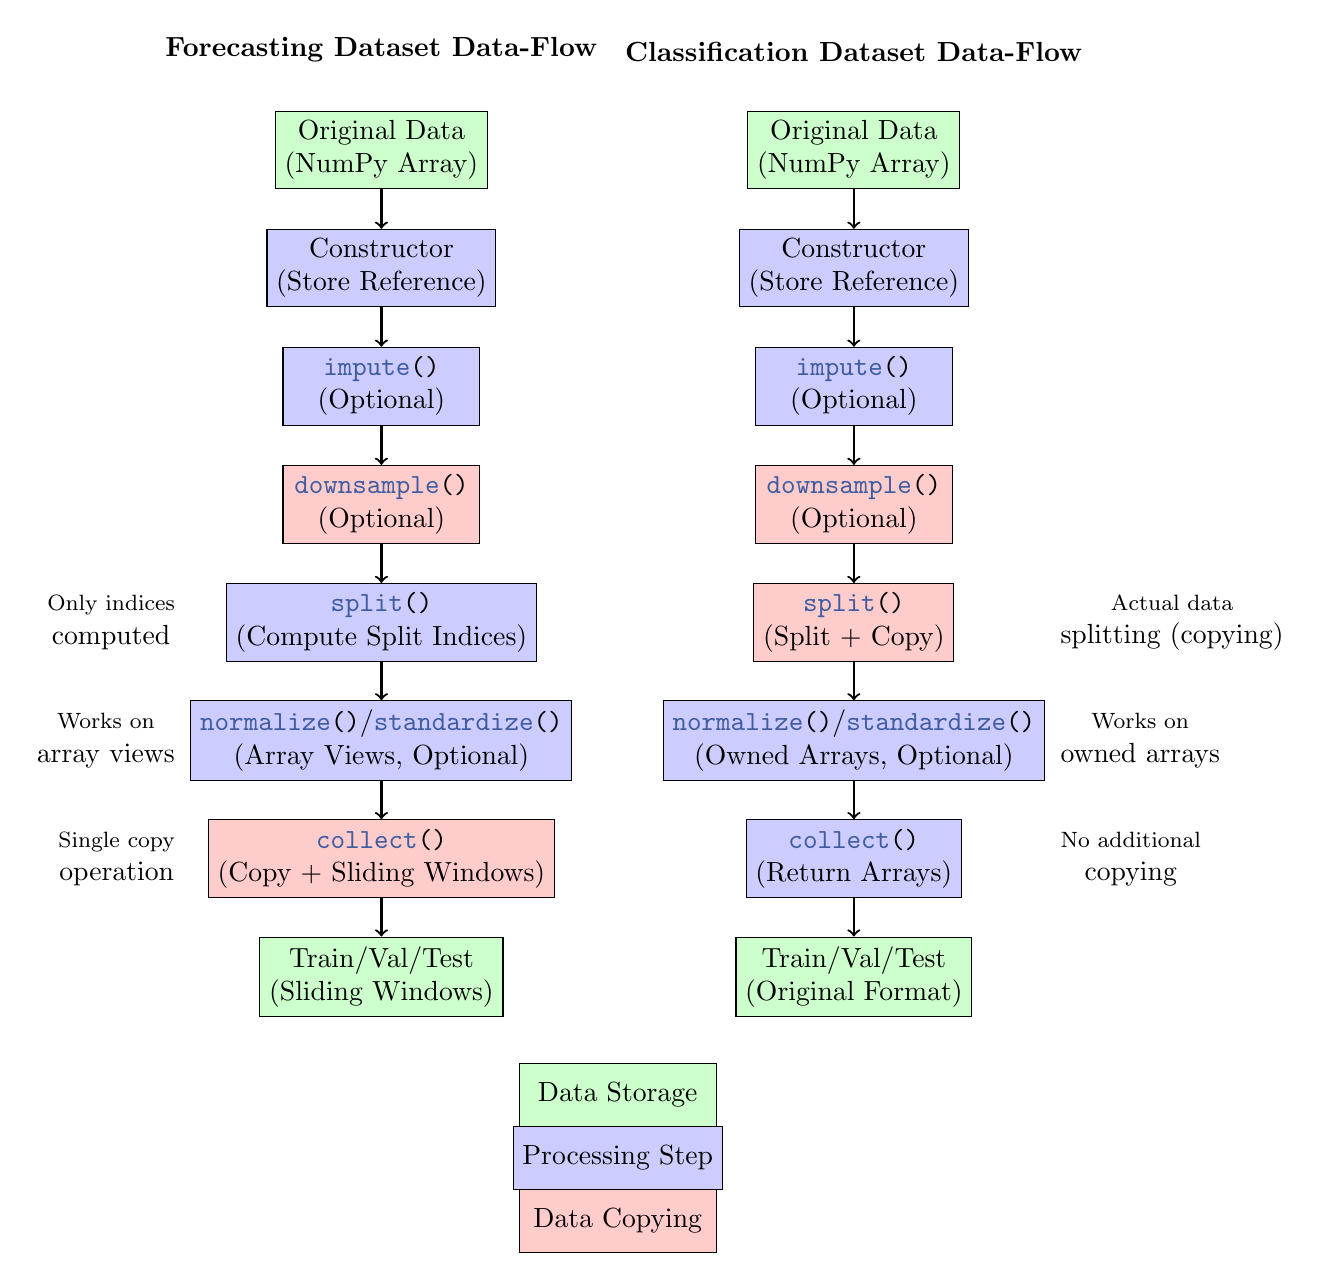
\begin{tikzpicture}[
            node distance=1.5cm,
            every node/.style={align=center},
            process/.style={rectangle, draw, fill=blue!20, minimum width=2.5cm, minimum height=0.8cm},
            data/.style={rectangle, draw, fill=green!20, minimum width=2.5cm, minimum height=0.8cm},
            decision/.style={diamond, draw, fill=yellow!20, minimum width=2cm, minimum height=0.8cm},
            arrow/.style={->, thick},
            dashedarrow/.style={->, thick, dashed},
            copy/.style={rectangle, draw, fill=red!20, minimum width=2.5cm, minimum height=0.8cm}    ]

        % Title
        \node[above] at (0, 8) {\textbf{Forecasting Dataset Data-Flow}};
        \node[above] at (6, 8) {\textbf{Classification Dataset Data-Flow}};

        % Forecasting flow (left side)
        \node[data] (f_data) at (0, 7) {Original Data\\(NumPy Array)};
        \node[process] (f_constructor) at (0, 5.5) {Constructor\\(Store Reference)};
        \node[process] (f_impute) at (0, 4) {\impute\\(Optional)};
        \node[copy] (f_downsample) at (0, 2.5) {\downsample\\(Optional)};
        \node[process] (f_split) at (0, 1) {\splitShort\\(Compute Split Indices)};
        \node[process] (f_normalize) at (0, -0.5) {\normalize/\standardize\\(Array Views, Optional)};
        \node[copy] (f_collect) at (0, -2) {\collect\\(Copy + Sliding Windows)};
        \node[data] (f_result) at (0, -3.5) {Train/Val/Test\\(Sliding Windows)};

        % Classification flow (right side)
        \node[data] (c_data) at (6, 7) {Original Data\\(NumPy Array)};
        \node[process] (c_constructor) at (6, 5.5) {Constructor\\(Store Reference)};
        \node[process] (c_impute) at (6, 4) {\impute\\(Optional)};
        \node[copy] (c_downsample) at (6, 2.5) {\downsample\\(Optional)};
        \node[copy] (c_split) at (6, 1) {\splitShort\\(Split + Copy)};
        \node[process] (c_normalize) at (6, -0.5) {\normalize/\standardize\\(Owned Arrays, Optional)};
        \node[process] (c_collect) at (6, -2) {\collect\\(Return Arrays)};
        \node[data] (c_result) at (6, -3.5) {Train/Val/Test\\(Original Format)};

        % Arrows for forecasting flow
        \draw[arrow] (f_data) -- (f_constructor);
        \draw[arrow] (f_constructor) -- (f_impute);
        \draw[arrow] (f_impute) -- (f_downsample);
        \draw[arrow] (f_downsample) -- (f_split);
        \draw[arrow] (f_split) -- (f_normalize);
        \draw[arrow] (f_normalize) -- (f_collect);
        \draw[arrow] (f_collect) -- (f_result);

        % Arrows for classification flow
        \draw[arrow] (c_data) -- (c_constructor);
        \draw[arrow] (c_constructor) -- (c_impute);
        \draw[arrow] (c_impute) -- (c_downsample);
        \draw[arrow] (c_downsample) -- (c_split);
        \draw[arrow] (c_split) -- (c_normalize);
        \draw[arrow] (c_normalize) -- (c_collect);
        \draw[arrow] (c_collect) -- (c_result);

        % Legend
        \node[data] at (3, -5) {Data Storage};
        \node[process] at (3, -5.8) {Processing Step};
        \node[copy] at (3, -6.6) {Data Copying};

        % Side annotations
        \node[left] at (-2.5, 1) {\footnotesize Only indices\\computed};
        \node[left] at (-2.5, -0.5) {\footnotesize Works on\\array views};
        \node[left] at (-2.5, -2) {\footnotesize Single copy\\operation};

        \node[right] at (8.5, 1) {\footnotesize Actual data\\splitting (copying)};
        \node[right] at (8.5, -0.5) {\footnotesize Works on\\owned arrays};
        \node[right] at (8.5, -2) {\footnotesize No additional\\copying};

    \end{tikzpicture}
    \caption{Data-flow comparison between forecasting and classification datasets. Red boxes indicate where data copying occurs, blue boxes indicate where data is processed without copying. Green boxes represent Python-side data storage.}
    \label{fig:data-flow-comparison}
\end{figure}

Why it is necessary to copy data in the \downsample step is explained in the \todo{Insert reference to downsample section}.

\subsection{Integration with LightningDataModule}

To make the library usable in a machine learning context, we integrated it with the PyTorch Lightning framework. This allows users to easily use our library in their machine learning pipelines, with the user not even having to understand our libraries interface. The integration is done by implementing a class that inherits from the \lightningDM class, which is the base class for all Lightning data modules. Such a \lightningDM can then be used in the \lightningModule as a data source. The \lightningModule offers a unified interface for simplifying machine learning workflows. Our class is called \rustDM, and it provides a simple interface to use our library in a Lightning context.

The user only ever needs to interact with the \rustDM class by passing the data as a \numpy array to the constructor, along with all parameters that let him choose which optional preprocessing features should be used, how the data should be split, and so on. No knowledge about the internal workings of the Rust implmentation is required. The user can then use the \rustDM class in the \lightningModule as a data source, and the data will be automatically prepared for usage in the machine learning pipeline. The signature of the \rustDM constructor looks as follows:

\begin{figure}[H]
    \begin{lstlisting}[
        style=python, 
        classoffset=4, 
        morekeywords={normalize, standardize}, 
        classoffset=2, 
        deletekeywords={normalize, standardize}
    ]
def __init__(
    self,
    dataset: np.ndarray,
    dataset_type: DatasetType,
    past_window: int = 1,
    future_horizon: int = 1,
    stride: int = 1,
    labels: np.ndarray | None = None,
    batch_size: int = 32,
    num_workers: int = 0,
    downsampling_rate: int = 0,
    normalize: bool = False,
    standardize: bool = False,
    impute_strategy: ImputeStrategy = ImputeStrategy.LeaveNaN,
    splitting_strategy: SplittingStrategy = SplittingStrategy.Temporal,
    splitting_ratios: tuple = (0.7, 0.2, 0.1),  # Train, validation, test ratios
):
...
    \end{lstlisting}
    \caption{Signature of the \rustDM constructor}
    \label{fig:rustdm-signature}
\end{figure}

The reference to the \numpy array, along with all options, are saved to the class. At the appropriate time, when the data modules \setup method is called, an instance of the appropriate class\\
(\forecastingDataSet or \classificationDataSet) is created, and the data is passed to it. All preprocessing methods are called according to the chosen options. The resulting split data is then again stored to the \rustDM class. It can be retrieved in the form of a PyTorch \dataLoader, which is a standard way to load data in PyTorch. The \dataLoader is used automatically by the \lightningModule to load the different parts of the data.

\newpage
\section{Random and Temporal Splitting}
With this library, we provide a simple and efficient way to split time series datasets into the three training, validation, and test sets. We support both random and temporal splitting.

Random splitting is useful for datasets where the order of the data points does not matter like in classification data, while temporal splitting is essential for time series data where the order is crucial like in the forecasting data.

List of supported splitting methods:
\begin{itemize}
    \item classification data : random splitting AND temporal splitting
    \item forecasting data : temporal splitting
\end{itemize}

When calling the function \splitShort we would need to pass four parameters:
\begin{itemize}
    \item \splitStrategy: the splitting strategy to use.
    \item \trainProp: the proportion of the training set, which is a float between 0 and 1.
    \item \valProp: the proportion of the validation set, which is a float between 0 and 1.
    \item \testProp: the proportion of the test set, which is a float between 0 and 1.
\end{itemize}

As we can see the pipeline of \textbf{random splitting} in \autoref{fig:random_split}, the steps are as follows:
\begin{enumerate}
    \item Validate the proportions of the training, validation, and test sets.
    \item Compute the number of instances in the dataset.
    \item Compute the split offsets for the training, validation, and test sets.
    \item Shuffle the dataset.
    \item Split the dataset into the three sets.
    \item Return the training, validation, and test sets.
\end{enumerate}

\begin{figure}
    \centering
    \includegraphics[width=1\textwidth]{files/splitting/random_split.png}
    \caption{Random Splitting}
    \label{fig:random_split}
\end{figure}

In case of \textbf{temporal splitting}, as shown in \autoref{fig:temporal_split}, we follow a similar approach, but we do not shuffle the dataset. The steps are as follows:
\begin{enumerate}
    \item Validate the proportions of the training, validation, and test sets.
    \item Compute the number of timesteps in the dataset.
    \item Compute the split offsets for the training, validation, and test sets.
    \item Split the dataset into the three sets.
    \item Return the training, validation, and test sets.
\end{enumerate}

\newpage

\begin{figure}
    \centering
    \includegraphics[width=1\textwidth]{files/splitting/temporal_split.png}
    \caption{Temporal Splitting}
    \label{fig:temporal_split}
\end{figure}

A code snippet of how one may use the splitting method is shown in \autoref{fig:usage_splitting}.

\begin{figure}[H]
    \begin{lstlisting}[style=python]

classification_data_set.split(SplittingStrategy.Temporal, 0.7, 0.2, 0.1)
    \end{lstlisting}
    \caption{Usage of the \splitShort method for \classificationDataSet}
    \label{fig:usage_splitting}
\end{figure}

\newpage
\section{Standardization and Normalization}
Another important step in preprocessing time series data is standardization and normalization.

Standardization is the process of scaling the data to have a mean of 0 and a standard deviation of 1, while min-max normalization scales the data to a range between 0 and 1.

We perform these two operations distinctly on each column of the dataset, which is essential for time series data where each column represents a different feature.

It is also worth mentionaning that key features such as mean, standard deviation, min, and max are computed only once for the training set and then applied to the validation and test sets. This is crucial to avoid data leakage, which can lead to overfitting and unrealistic performance metrics.

\subsection{Standardization}

Standardization is performed by subtracting the mean and dividing by the standard deviation for each feature. This ensures that the data has a mean of 0 and a standard deviation of 1.

Here are the main steps of the standardization process:
\begin{enumerate}
    \item Compute the mean and standard deviation for each feature in the training set.
    \item Through a for loop iterate over each feature and apply the standardization formula:
          \begin{equation}
              x' = \frac{x - \text{mean}}{\text{std}}
          \end{equation}
    \item Apply the same mean and standard deviation to the validation and test sets.
\end{enumerate}

\subsection{Min-Max Normalization}
Min-max normalization scales the data to a range between 0 and 1. This is particularly useful for algorithms that are sensitive to the scale of the data, such as neural networks.

Here are the main steps of the min-max normalization process:
\begin{enumerate}
    \item Compute the minimum and maximum values for each feature in the training set.
    \item Through a for loop iterate over each feature and apply the min-max normalization formula:
          \begin{equation}
              x' = \frac{x - \text{min}}{\text{max} - \text{min}}
          \end{equation}
    \item Apply the same min and max values to the validation and test sets.
\end{enumerate}

In the bottle neck scenario, where the difference between the minimum and maximum values is zero, we set their values to 1, which avoids division by zero errors.

A code snippet of how one may use the standardization and normalization methods is shown in \autoref{fig:usage_standardization_normalization}.
\begin{figure}[H]
    \begin{lstlisting}[style=python]
classification_data_set.normalize()
classification_data_set.standardize()
    \end{lstlisting}
    \caption{Usage of the standardization and normalization methods}
    \label{fig:usage_standardization_normalization}
\end{figure}

\newpage
\section{Downsampling}
Downsampling is the process of reducing the number of data points in a time series dataset. This is useful for reducing the size of the dataset and speeding up the training process, especially when dealing with large datasets.

When calling the function \downsample, we need to pass one parameter:
\begin{itemize}
    \item \factor: the factor by which to downsample the dataset, which is an integer greater than 1.
\end{itemize}

The downsampling process works by taking every \factor-th data point in the dataset. For example, if the factor is 2, we take every second data point, effectively halving the size of the dataset.

An illustration of how downsampling with \factor 2 works is shown in \autoref{fig:downsampling}.
\begin{figure}
    \centering
    \includegraphics[width=0.8\textwidth]{files/downsampling/downsampling.png}
    \caption{Downsampling}
    \label{fig:downsampling}
\end{figure}

In the Rust side, we loop through the dataset and create a new dataset with only the data points that are at indices that are multiples of the downsampling factor. This is done efficiently using the \texttt{ndarray} library.

A code snippet of how one may use the downsampling method is shown in \autoref{fig:usage_downsampling}.
\begin{figure}[H]
    \begin{lstlisting}[style=python]
classification_data_set.downsample(2)
    \end{lstlisting}
    \caption{Usage of the downsampling method}
    \label{fig:usage_downsampling}
\end{figure}

\newpage
\section{Imputing}

\newpage
\section{Testing}
We have implemented unit tests for nearly all the methods in the library. These tests cover various scenarios and edge cases to ensure the correctness of the implementation.

Since our rust code is deeply integrated with bindings and the the Pyo3 library, we were not able to write pure Rust tests. Instead, we have mimicked python environment in the Rust tests, which allows us to test the methods as if they were called from Python.
We did this by using the \texttt{pyo3} library, which allows us to write Python code in Rust and test it as if it were called from Python.

One might wonder why we did not use the \texttt{pytest} library to test the Python code directly. The reason is that we wanted to ensure that the Rust code is working correctly and that the bindings are working as expected. This way, we can catch any issues in the Rust code before they propagate to the Python side.
Also, there were some functions that were not directly callable from Python, as they were private functions in the Rust code. We wanted to test these functions as well, so we had to write tests in Rust and compile them differently from how we compiled for the Python bindings.

\subsection{Running the Tests}
To run the tests, we would need to follow these steps:
\begin{enumerate}
    \item One may want to clean up all the build artifacts from previous builds. This can be done by running the following command:
          \begin{verbatim}cargo clean
    \end{verbatim}
    \item Ensure that the \texttt{maturin} library is installed. This can be done by running the following command:
          \begin{verbatim}pip install maturin
    \end{verbatim}
    \item Now build the Rust code with the \texttt{test\_expose} feature enabled. This can be done by running the following command:
          \begin{verbatim}maturin develop --features test_expose
    \end{verbatim}
    \item (Only on Mac) Find the location of the \texttt{libpython3.12.dylib} file. This can be done by running the following command:
          \begin{verbatim}find $(python3 -c "import sys; print(sys.prefix)") -name "libpython3.12.dylib"
    \end{verbatim}
    \item (Only on Mac) Set the \texttt{DYLD\_LIBRARY\_PATH} environment variable to the path of the \texttt{libpython3.12.dylib} file. This can be done by running the following command:
          \begin{verbatim}export DYLD_LIBRARY_PATH=given_path_from_above
    \end{verbatim}
    \item Finally, run the tests with the following command:
          \begin{verbatim}cargo test --features test_expose
    \end{verbatim}
\end{enumerate}

\subsection{Test Coverage}
As also mentioned above, we have implemented the unit tests through mimicking the Python environment in Rust.
This came with some down sides, which doesn't allow us to use the \texttt{cargo-tarpaulin} library to measure the test coverage.
However, we have manually checked the coverage of the tests and ensured that all the methods are covered by the tests. We have also ensured that the tests cover various scenarios and edge cases to ensure the correctness of the implementation.

In order to have a rough estimate of the test coverage, we have counted the number of all the functions in the library and the number of functions that are covered by the tests.

The results are as follows:
\begin{itemize}
    \item Total number of functions(excluding bindings): 41
    \item Number of test cases: 34
    \item Test coverage: \textbf{83\%}
\end{itemize}

Please note that this is a rough estimate and the actual test coverage may vary. We have also ensured that the tests cover various scenarios and edge cases to ensure the correctness of the implementation.

\newpage
\section{Benchmarking}
\newpage
\pagestyle{empty}

\includepdf[pages=-,pagecommand={},width=\textwidth]{files/oathstatement.pdf}

\newpage
\pagestyle{empty}

\includepdf[pages=-,pagecommand={},width=\textwidth]{files/oathstatement.pdf}

\newpage
\pagestyle{empty}

\includepdf[pages=-,pagecommand={},width=\textwidth]{files/oathstatement.pdf}

\end{document}
